We describe the choices we did about representation of the data and communication between modules.
These choices are described precisely in the documentation\footnote{\url{https://github.com/ProjetPP/Documentation/}} of the project.

\section{Data model}
\label{rdf}

First, we present the data model. Its aim is to represent in a well formatted structure all data submit to or generate by the modules. It must be able to contain raw data (as the input sentence or an output description) as well as structured data (as a parsed question). We will begin by describe the abstract structure without detail of implementation and justify this choice.

\subsection{Abstract structure}

The data model is very close of the first order logic. We will define recursively the structure.

A basic element is called \textsl{\bf resource}. A \textsl{resource} represent a string, an integer, coordinates etc.. \textsl{Resources} can theoretically be in infinite number, even in uncountable number (but, for obvious reason, computer cannot handle such sets).

We define a \textsl{\bf list} as a finite sequence of \textsl{resources}. We identify the \textsl{list} \textsl{(a)} and the resource \textsl{a}. The use of this identification will be explained later. Moreover, a \textsl{list} must have no duplicates. For instance \textsl{[a,a]} is not a list and need to be simplify as \textsl{[a]}. We can see \textsl{lists} as finite totally ordered set.

The other atomic elements are the boolean values \textsl{\bf true} and \textsl{\bf false}. They are not \textsl{resources} as previously defined. Nevertheless, we admit \textsl{resources} "true" and "false" but we cannot apply logic operation on them.

A \textsl{triple} is a 3-tuple containing in this order:
\begin{itemize}
    \item a subject: what the triple refers to,
    \item a predicate: the relation between the subject and the object,
    \item an object: what the property of the subject refers to.
\end{itemize}
For instance, we can represent the sentence "Isaac \textsc{Newton} is born the 25 December 1642 (Julian)" by the triple \begin{center}(Isaac \textsc{Newton}, birth date, 25 December 1642 (Julian))\end{center}


The is so reasonable to associate to each triple a boolean value depending upon whether the triple state a truth or not. Generally triples contains \textsl{lists} with more than one value. So we define the node \textsl{full triple} 
\begin{center}
\textsl{full triple: list$^3\rightarrow$ bool}
\end{center}
and we define the value of a full triple \textsl{(a,b,c)} as $$(a,b,c)=\bigwedge_{i=1}^{n_a}\bigwedge_{j=1}^{n_b}\bigwedge_{k=1}^{n_c} (\textsl{a}_i,\textsl{b}_j,\textsl{c}_k)$$where $a=[a_1,\ldots,a_{n_a}]$, $b=[b_1,\ldots,b_{n_b}]$ and $c=[c_1,\ldots,c_{n_c}]$.

This structure is needed to check if a statement is true. That naturally correspond to yes/no questions.

A kind of natural yes/no question which are not handled by \textsl{full triple} are existential questions: "Is there a... ?". To represent them, we use a node \textsl{exists} (also denoted by $\exists$)
\begin{center}
\textsl{exists: list$\rightarrow$ bool}
\end{center}
and the evaluations is \textsl{exists$(l) = \begin{cases}
\textsl{true} & \text{if }l\neq\emptyset\\
\textsl{false} & \text{if }l=\emptyset
\end{cases}$}. This node checks whether the list is non empty.

Of course, we allow all boolean operations as node: and ($\wedge$), or ($\vee$), not ($\neg$)\dots.

\bigskip

Now we define operations on \textsl{lists}.

We have natural operation like union, intersection, difference\ldots.

We also allow \textsl{incomplete triples}. An incomplete triple is a triple with a "hole": we know only two values and we want the list of all values which satisfy the triple. There is 3 type of required triples: for subject, predicate and object. They have the type
\begin{center}
\textsl{incomplete triple: list$^2\rightarrow$ list}
\end{center}
and the evaluations are
\begin{itemize}
    \item for subject: $\textsl{incomplete triple}_{\textsl{subject}}(a,b) = \textsl{list}(\{\textsl{x}\mid(x,a,b)\})$ denoted by $(?,a,b)$,
    \item for predicate: $\textsl{incomplete triple}_{\textsl{predicate}}(a,b) = \textsl{list}(\{\textsl{x}\mid(a,x,b)\})$ denoted by $(a,?,b)$,
    \item for object: $\textsl{incomplete triple}_{\textsl{object}}(a,b) = \textsl{list}(\{\textsl{x}\mid(a,b,x)\})$ denoted by $(a,b,?)$.
\end{itemize}

We define to additional nodes: \textsl{sort}, \textsl{first} and \textsl{last}.

\begin{center}
\textsl{sort: list$\times$resource$\rightarrow$list}
\end{center}
This function \textsl{sort} take a list and a predicate and sort the element of the list in the increasing order according to the value returned by the predicate. More formally, let $l=[l_1,\ldots,l_n]$, $p$ a predicate and $a_i$ such that $\forall i\in\llbracket1,n\rrbracket, (l_i,p,a_i)$. Then, \textsl{sort}$(l,p) = [l_{\sigma(1)},\ldots,l_{\sigma(n)}]$ where $\sigma\in\mathfrak{S}_n$ and $\forall (i,j)\in\llbracket 1,n\rrbracket^2, \sigma(i)<\sigma(j) \Leftrightarrow a_i \leqslant a_j$. This definition need all sets are totally ordered. In this case, that is reasonable, even if order are not really clever.

All previous operations have no specification about the order.

The function \textsl{first} returns the first (smallest if the list is ordered) element of a list.

The function \textsl{last} returns the last (greatest if the list is ordered) element of a list.

\subsection{Examples}

To clarify the previous definitions, we give some examples.

\bigskip

"Is Isaac \textsc{Newton} born the 25 December 1642 (Julian)?"
\begin{center}(Isaac \textsc{Newton}, birth date, 25 December 1642 (Julian))\end{center}

\bigskip

"Is Isaac \textsc{Newton} born the 25 December 1642 (Julian) and dead the 20 Marsh 1727 (Julian)?"
\begin{center}(Isaac \textsc{Newton}, birth date, 25 December 1642 (Julian))$\wedge$(Isaac \textsc{Newton}, death date, 20 Marsh 1727 (Julian))\end{center}

\bigskip

"Who were the presidents of the United States?"
\begin{center}(United States, president, ?)\end{center}

\bigskip

"Who is mayor of the capital of Kreis Bergstraße?"
\begin{center}((Kreis Bergstraße, capital, ?), mayor, ?)\end{center}

\bigskip

"Who are the daughters of the wife of the husband of the wife of the president of the United States?"
\begin{center}
(((((United States, president,?), wife, ?), husband, ?), wife, ?), daughter, ?)
\end{center}

\bigskip

"What is the birth date of the first president of the United States?"
\begin{center}(first((United States, president, ?), mandate begin date), birth date, ?)\end{center}

\bigskip

"Is there a medical treatment for ebola?"
\begin{center}\textsl{exists}((ebola, medical treatment, ?))\end{center}

\bigskip

"Who are the children of Nicolas \textsc{Sarkozy} and Carla \textsc{Bruni}?"
\begin{center}(Nicolas \textsc{Sarkozy}, child, ?)$\cap$(Carla \textsc{Bruni}, child, ?)\end{center}

\subsection{Software point of view}

All normalised structures of the PPP are JSON-serializable, i.e. they are trees made of instances of the following types:
\begin{itemize}
    \item \texttt{Object}
    \item \texttt{List}
    \item \texttt{String}
    \item \texttt{Number}
    \item \texttt{Boolean}
    \item \texttt{Null}
\end{itemize}

We chose to represent all normalised data as trees. We use the previous nodes and we represent the '?' in incomplete triples.

The node \texttt{resource} to represent the previous abstract node \textsl{resource} and \textsl{bool}. Moreover, we identify the \textsl{resource} "true" and the boolean value \textsl{true} and the same for "false" and "false". This identification is not problematic for type because we assume modules creates only well-formed expressions.

We add to the nodes we defined above some new features:
\begin{itemize}
    \item a \texttt{sentence} node: a question in natural language like "Who is George Washington?",
    \item we can precise a type to \texttt{resource} and \texttt{missing} nodes. For example, if we choose as range "time" to the missing node ? in the triple (George Washington, birth, ?) this triple with hole can only return time points.
\end{itemize}

For example, the work of the question parsing module is to transform 
\begin{verbatim}
{
    "type": "sentence", 
    "value": "Who is George Washington?"
}
\end{verbatim}
into 
\begin{verbatim}
{
    "type":
        "triple",
    "subject":{
        "type": "resource",
        "value": "George Washington"
    },
    "predicate":{
        "type": "resource",
        "value": "identity"
    },
    "object":{
        "type": "missing"
    }
}
\end{verbatim}

The basic value types are 
\begin{itemize}
    \item \texttt{string},
    \item \texttt{boolean},
    \item \texttt{time},
    \item \texttt{math-latex} (for mathematical formulas written with \LaTeX),
    \item \texttt{geo-json} (for geographic data).
\end{itemize}

\section{Communication}

Modules communicate with the core via HTTP requests.

The core sends them a JSON object, and they return another one.

The basic idea is that the core iterates requests to modules, which return a simplified tree, until the core gets a complete response, ie. a tree without any `missing` node.

During these exchanges, we keep a trace of the different steps between the original request and the current tree. The structure of a trace is a list of such trace items:
\begin{verbatim}
{
    "module":
        "<name of the module>", 
    "tree":{
        <answer tree>
    },
    "measures":{
        "relevance": <relevance of the answer>,
        "accuracy": <accuracy of the answer>
    }
}
\end{verbatim}

The measure field contains two values: relevance and accuracy.

\begin{itemize}
    \item \texttt{accuracy} is a self-rating of how much the module may have correctly understood (ie. not misinterpreted) the request/question. It is a float between 0 and 1.
    \item \texttt{relevance} is a self-rating of how much the tree has been improved (i.e. progressed on the path of becoming a useful answer). A positive float (not necessarily greater that 1; another module might use it to provide a much better answer).
\end{itemize}

We do not provide a method to compute these values. We have to trust every modules.

This form allows each module to access to the previous results, particularly to the request of the user. The objects for request and response contain some extra data, such as the language used.

We can use these measure to chose the best answer to display it at the first position in the UI. Modules can use them to. For instance, if there is two modules for question parsing, a module will choose one of the two answers based on these marks.

The data model have been implemented in a nice set of objects in both Python\footnote{\url{http://github.com/ProjetPP/PPP-datamodel-Python/}} and PHP\footnote{\url{http://github.com/ProjetPP/PPP-datamodel-PHP/}} in order to help the writing of modules.

We could define a linear representation for the trace, using the representation of the datamodel, but it is not relevant. Indeed, this information will never be printed on the user interface.

\begin{figure}[!ht]
% https://docs.google.com/drawings/d/1toUH24GqwtpvKV7S5gje6GBxfa13R3mxgm8WlAFc_0g/edit?usp=sharing
  \centering
    \label{datamodel:struct}
    \caption{Architecture of the PPP}
    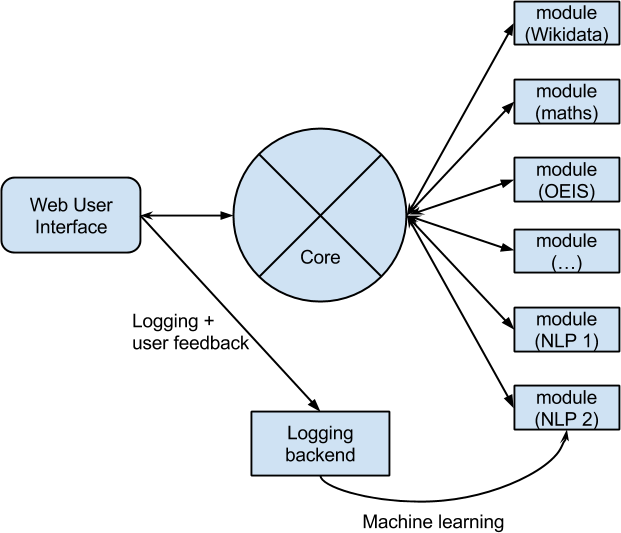
\includegraphics[width=0.8\textwidth]{../ppp_structure.png}
\end{figure}

\section{Evolution of data model}

In the first version of the data model, there were only incomplete triples. The semantic power is intrinsically lower. In particular, this model can't represent yes/no questions.